\section{결과 및 토의}

우선 온습도센서는 프로그램을 실행하였을 때 정상적으로 온도와 습도가 표현됨을 알 수 있었으나 기압센서는 SPI 통신을 사용하였을 때 기압이 약 390hPa 정도로 실제와 전혀 맞지 않는 값이 출력되었다. 센서를 교체하여도 같은 현상이 일어났고 센서에서 값을 받아오는 것 자체에는 문제가 없는 것으로 판단되었으므로 센서에서 받아온 값을 기압으로 출력하는 명령어에 문제가 있던 것으로 추정된다. 그러나 SPI 통신은 ADC가 사용하여야 하고 라즈베리파이 하나에는 기본적으로 한 세트의 SPI 통신 판만이 존재하기에 대신 I2C 통신을 사용하여 기압센서를 연결하였으며, 그 결과 기압이 1000mba 내외로 정상적으로 표출되어서 기압 값을 수집할 때 I2C 통신을 사용하기로 하였다. 

미세먼지 센서의 경우 프로그램이 실행된 이후 몇 초 동안은 값이 정상적으로 표출되었으나 그 후 원인불명의 오류와 함께 프로그램이 정지하였다. UART 통신에서 값을 받아오는 부분에 문제가 있던 곳으로 추정되며 일반적인 자동기상관측장비에서는 미세먼지 농도를 측정하지 않기에 AWS에 미세먼지 센서는 일단 설치하지 않는 것으로 결정하였다. 

ADC의 경우 C언어와 Python으로 컴파일된 프로그램 두 개를 각각 실행한 결과 Python 코드의 경우 오류는 발생하지 않으나 센서의 연결 여부와 무관하게 전압이 계속 0으로 측정되는 문제가 있었다. 반면 C언어 코드의 경우 전압이 정상적으로 출력되었다. AWS를 구동하는 전체 명령어는 Python으로 작성하였으므로 C언어에서 파일 입출력을 통해 텍스트 파일에 수집한 전압 값을 Python에서 다시 한 줄씩 읽어들이는 방법을 선택하였다. 풍속 센서의 경우 라즈베리파이에 (+)극과 GND를 연결하지 않으며 오로지 출력 전압을 연결하는 핀 하나만 ADC에 연결한다. 

그렇기 때문에 라즈베리파이에 전원을 공급하는 배터리와 풍속 센서에 전원을 공급하는 배터리가 같아야 두 장치에 연결된 GND의 전위가 같아 값이 정상적으로 표현된다. 1.5V 건전지의 (-)극은 라즈베리파이의 GND에, (+)극은 ADC에 연결하였을 때 약 1350mV 정도의 값이 출력되었으며 건전지의 내부 저항을 고려하면 타당한 값으로 생각된다. 

풍속 센서의 출력 전압이 0.4V일 때의 풍속이 0m/s임이 데이터시트에 명시되어 있었으므로 0.4V 전압 이하에서의 풍속을 0으로 가정하였다. 풍향 센서의 경우 12V 전원을 공급한 후 풍향계가 향하는 방향을 달리한 뒤 멀티미터를 사용하여 배터리의 GND와 출력 핀 사이의 전압을 측정한 결과 방향과 무관하게 10V 가량이 나왔다. 데이터시트에 의하면 풍향에 따라 최대 5V의 전압이 출력되어야 하므로 잘못된 값임을 알 수 있다. 

강우량 센서의 경우 물방울이 한 번 떨어질 때마다 프로그램을 실행한 이후의 누적 강우량이 정상적으로 출력되었다. 최종 프로그램을 실행하였을 때 온습도와 기압, 단위 시간당 강우량, 풍속이 MariaDB 서버 데이터베이스에 정상적으로 전송됨을 확인하였다.

\begin{figure}[htbp]
	\centering
	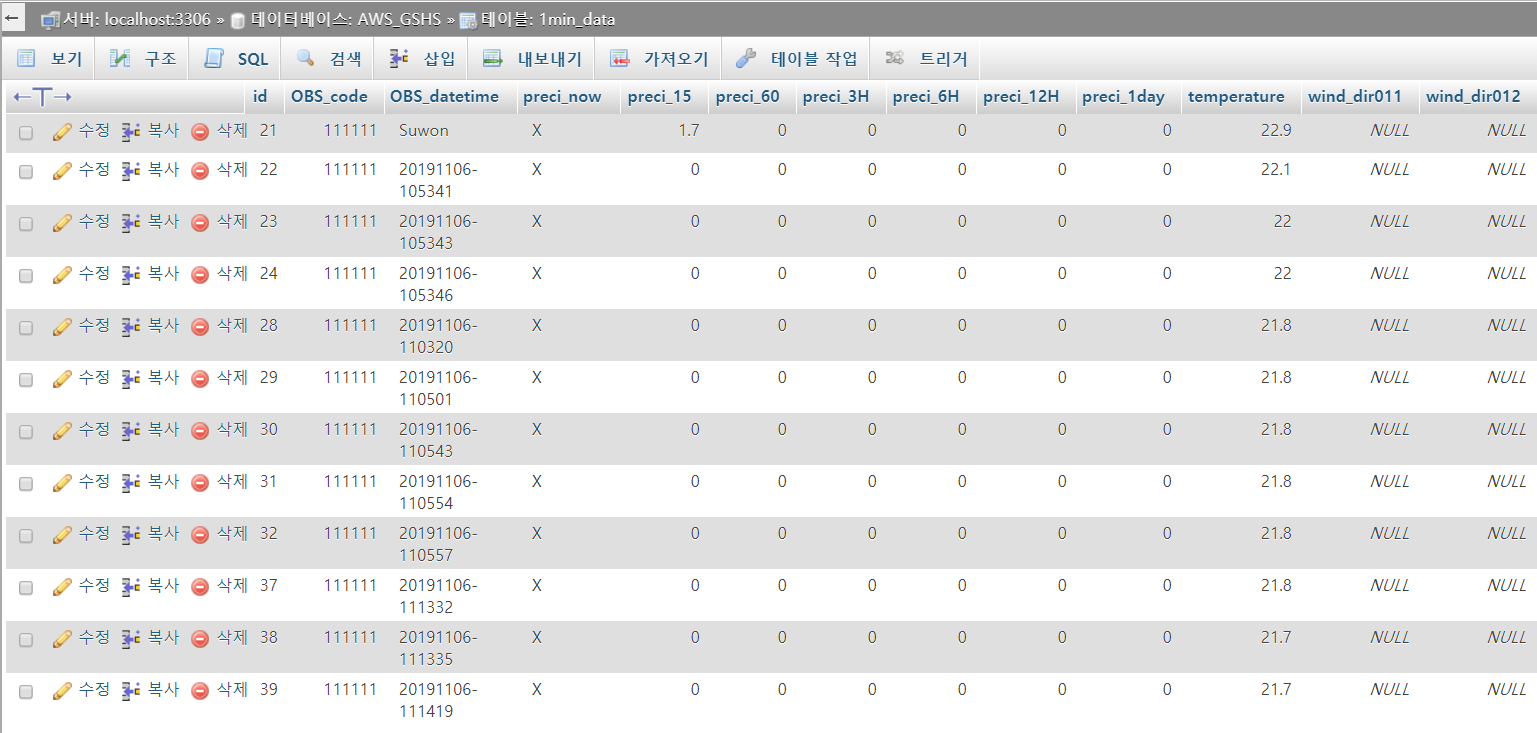
\includegraphics[width=.9\textwidth]{dbsuccess.png}
	\caption{측정한 기상 정보를 DB에 전송한 모습}
	\label{DBSENT}
\end{figure}

\begin{figure}[htbp]
	\centering
	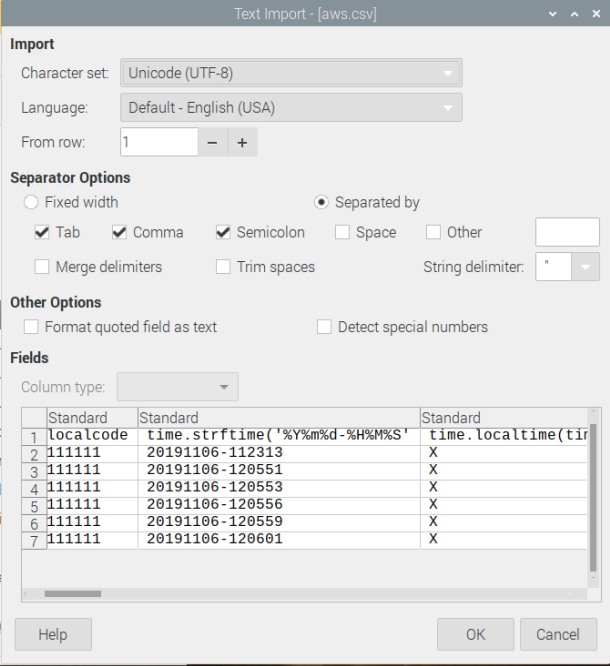
\includegraphics[width=.7\textwidth]{awscsv}
	\caption{라즈베리파이 내부 저장소에 저장된 데이터}
	\label{AWSCSV}
\end{figure}